\documentclass[11pt,a4paper]{article}
\usepackage[T1]{fontenc}
\usepackage[utf8]{inputenc}
\usepackage[english]{babel}
\usepackage{lmodern}
\usepackage{microtype}
\usepackage{amsmath,amssymb,amsthm,mathtools}
\usepackage{geometry}
\usepackage{enumitem}
\usepackage{booktabs}
\usepackage{hyperref}
\usepackage{tikz}
\usetikzlibrary{automata,positioning,arrows.meta}
\geometry{margin=2.5cm}

\newtheorem{definition}{Definition}[section]
\newtheorem{proposition}[definition]{Proposition}
\newtheorem{theorem}[definition]{Theorem}
\newtheorem{lemma}[definition]{Lemma}
\newtheorem{remark}[definition]{Remark}

\newcommand{\Nat}{\mathbb{N}}
\newcommand{\Stream}[1]{#1^\omega}
\newcommand{\True}{\mathsf{true}}
\newcommand{\False}{\mathsf{false}}
\newcommand{\StepRel}{\mathsf{Step}}
\newcommand{\Cfg}{\mathsf{Cfg}}
\newcommand{\Obs}{\mathsf{Obs}}
\newcommand{\TickCtx}{\mathsf{TickCtx}}
\newcommand{\UserInv}{\mathsf{Inv}}
\newcommand{\Match}{\mathsf{Match}}
\newcommand{\BadLocal}{\mathsf{BadLocal}}
\newcommand{\GeneratedBy}{\mathsf{GeneratedBy}}
\newcommand{\AvoidA}{\mathsf{AvoidA}}
\newcommand{\AvoidG}{\mathsf{AvoidG}}
\newcommand{\run}{\mathsf{run}}
\newcommand{\rps}{\mathsf{rps}}
\newcommand{\ctx}{\mathsf{ctx}}
\newcommand{\head}{\mathsf{hd}}
\newcommand{\tail}{\mathsf{tl}}

\title{Safety Automata, Explicit Products, and Local Clauses for Kairos}
\author{Kairos Project}
\date{\today}

\begin{document}
\maketitle

\begin{abstract}
Kairos aims to prove that a reactive program satisfies a safety guarantee for
all inputs admitted by an environment hypothesis. The difficulty is that the
target property is global and ranges over infinite traces, whereas external
proof tools ultimately validate transition-level Hoare triples built from local
semantic clauses. This document presents the semantic object that connects
these two levels: the
explicit product of the program, the assumption automaton, and the guarantee
automaton. We give a rigorous definition of the program, its stream semantics,
safety automata, and node invariants over trace contexts. We then explain how a
concrete tick realizes an abstract product step, why some steps are dangerous,
and how local clause generation should be read as a static construction over
such steps before being assembled into relational Hoare triples. Finally, we
align this presentation with the Rocq formalization and with the current
Kairos implementation.
\end{abstract}

\section{Introduction}
Reactive programs are naturally specified over traces. In the setting studied
here, a program is executed under an environment hypothesis on input streams,
and its correctness is expressed by a safety guarantee on the resulting
input/output trace. The user may also supply node invariants that capture
additional semantic facts about executions. The resulting specification is
therefore not a simple assertion over isolated states, but a conditional
property over infinite reactive behaviors.

The mathematical difficulty is that the specification lives at two different
scales. On the one hand, assumptions and guarantees are properties of complete
traces, usually presented through safety automata. On the other hand, the local
reasoning principles used to justify the absence of bad executions are attached
to individual ticks and finite transitions. A satisfactory mathematical account
must therefore explain how one moves from infinite-word semantics to local
clauses and transition triples without losing the meaning of the original conditional safety
statement.

This paper develops that account around one central object: the explicit
product \(program \times A \times G\), where \(A\) is the assumption automaton
and \(G\) is the guarantee automaton. The product is the semantic object that
synchronizes, at each tick, a program transition, the reading of the current
input by \(A\), and the reading of the current observation by \(G\). Once this
product is available, one can characterize dangerous steps, namely product
steps that remain within the admissible input domain while taking the guarantee
to its bad state. Local clauses are then understood as static formulas
generated from these abstract steps. The purpose of the construction is to make
precise a reduction of the following shape: if a complete execution violates
the guarantee under admissible inputs, then some concrete tick realizes a
dangerous product step, and the corresponding local safety clause is false.

The first contribution of the paper is a precise mathematical model of reactive
programs, executions on streams, trace-derived local contexts, deterministic
safety automata, and node invariants over such contexts. The second
contribution is a formal presentation of the explicit product and of the local
matching relation between abstract product steps and concrete ticks. The third
contribution is a procedural and logical account of clause generation:
which semantic clauses are produced, from which static ingredients, how they
are assembled into relational Hoare triples, and how those triples
participate in the global safety argument. Although the focus of the paper is
mathematical, this model is also meant to clarify the structure later used by
the implementation. In particular, the mathematical core developed here stops
at validity of generated relational Hoare triples; actual external validation
is a later refinement layer.

The remainder of the paper is organized as follows. Section~2 defines reactive
programs, their stream semantics, and the local trace contexts on which
specifications are interpreted. Section~3 introduces deterministic safety
automata and the interpretation of local predicates, including predicates with
past. Section~4 presents the explicit product and its semantic role. Section~5
defines dangerous steps, local contexts, and the matching relation. Section~6
describes clause generation and triple assembly in a pseudo-algorithmic yet
formal way. Section~7 reconstructs the proof chain from a global bad execution
to the violation of a local safety clause. Section~8 discusses the connection between the
mathematical presentation and the current implementation architecture.

\section{Reactive Program and Stream Semantics}

\subsection{Reactive Program}

A Kairos program is viewed as a stateful reactive system. The program state
contains a control component and a memory component. Program transitions are not
written as imperative assignments, but as logical relations between the current
state, the current input, the current output, and the next state.

\begin{definition}[Reactive Program]
A reactive program \(P\) is given by:
\[
P = (S,M,I,O,T,s_0,m_0,\StepRel),
\]
where:
\begin{itemize}[leftmargin=1.4em]
\item \(S\) is the set of control states;
\item \(M\) is the set of memory states;
\item \(I\) is the set of inputs;
\item \(O\) is the set of outputs;
\item \(T\) is a set of transition identifiers;
\item \(s_0 \in S\) and \(m_0 \in M\) are the initial conditions;
\item \(\StepRel(t,s,m,i,s',m',o)\) is a logical predicate, read as:
  transition \(t\) allows the passage from \((s,m)\) to \((s',m')\) under
  input \(i\), producing output \(o\).
\end{itemize}
\end{definition}

\begin{definition}[Program Specification]
The specification associated with \(P\) is a triple
\[
\Phi = (A,G,\UserInv),
\]
where:
\begin{itemize}[leftmargin=1.4em]
\item \(A\) is a safety automaton over input streams;
\item \(G\) is a safety automaton over reactive input/output traces;
\item \(\UserInv : S \to (\TickCtx \to \mathsf{Prop})\) is an aggregated node
  invariant: for each control state \(s\), \(\UserInv(s)\) is a property over
  tick contexts compatible with the execution.
\end{itemize}
\end{definition}

\begin{remark}
The key point is the distinction between:
\begin{itemize}[leftmargin=1.4em]
\item the \emph{program} \(P\), which contains only its syntax and step
  semantics;
\item the \emph{specification} \(\Phi=(A,G,\UserInv)\), which contains the
  external hypotheses, the guarantee, and node formulas over the execution
  trace.
\end{itemize}
Kairos clauses therefore do not arise from an ``enriched program'' object,
but from the coupling of \(P\) and \(\Phi\).
\end{remark}

\subsection{Determinism and Step Relation}

To avoid unnecessary overhead, we work in the deterministic setting targeted by
Kairos: at each tick, the program selects a unique transition, and the automata
also select a unique outgoing edge.

\begin{definition}[Deterministic Program Step]
Assume a functional step relation such that, for every
\((s,m,i)\), there exists a unique triple \((t,(s',m'),o)\) satisfying
\[
((s,m),i)\xrightarrow{\,t\,}_P((s',m'),o).
\]
This relation is compatible with \(\StepRel\), namely:
\[
((s,m),i)\xrightarrow{\,t\,}_P((s',m'),o)
\Longrightarrow
\StepRel(t,s,m,i,s',m',o).
\]
\end{definition}

\begin{remark}[Totality Assumption on Program Ticks]
The abstract model used in this paper assumes that every instant is total: from
every current configuration and input valuation, the program computes a next
control state, a next memory, and an output valuation. This is stronger than
what a concrete implementation language may guarantee by construction. In
particular, a concrete program may block because of an invalid operation, or
fail to emit a value on some output signal. Such situations are intentionally
abstracted away from the mathematical core and must therefore be ruled out by
separate well-formedness conditions when one applies the model to actual Kairos
programs.
\end{remark}

\begin{remark}[Exhaustiveness of Transition Filtering]
Another practical source of non-totality is the absence of any active
transition for the current control state, memory, and input valuation. In the
abstract model, this case is excluded: the filtering of transitions by current
state and guard satisfaction is assumed to be exhaustive on the executions of
interest. In practice, this should be guaranteed structurally, for instance by
requiring exhaustive guarded cases or by inserting an explicit default branch
at the source-language level. Introducing a semantic sink state inside the
abstract program model would require specifying its observable output, which is
not neutral; for this reason, the present paper treats exhaustiveness as a
well-formedness requirement on concrete programs rather than as part of the
core semantics.
\end{remark}

\subsection{Stream Semantics}

A local transition is not enough: one must define the execution of the program
over an infinite input stream. This is where stream semantics comes in.

\begin{definition}[Stream]
For every set \(X\), we write
\[
\Stream{X} := \Nat \to X
\]
for the set of infinite streams over \(X\).
\end{definition}

\begin{definition}[Configuration and Observation]
We write
\[
\Cfg := S \times M,
\qquad
\Obs := I \times O.
\]
\end{definition}

\begin{definition}[Local Tick Context]
We define
\[
\TickCtx := \Nat \times \Cfg \times I \times O \times \Cfg.
\]
An element
\[
(k,(s,m),i,o,(s',m')) \in \TickCtx
\]
is called a \emph{local tick context}. It represents the smallest execution
window around tick \(k\): current configuration, current input, current output,
and next configuration.
\end{definition}

\begin{definition}[Trace-Derived Local Context]
Fix an input stream \(u \in \Stream{I}\), and let
\((s_u,m_u,o_u)\) be the execution generated by \(P\) on \(u\). We write
\[
\ctx_u(k) :=
\bigl(k,\,(s_u(k),m_u(k)),\,u(k),\,o_u(k),\,(s_u(k+1),m_u(k+1))\bigr)
\in \TickCtx,
\]
that is, the context obtained at tick \(k\) from the current configuration, the
current input, the current output, and the next configuration of the execution.
\end{definition}

\paragraph{Notation conventions.}
Fix an input stream \(u \in \Stream{I}\). The program \(P\) then generates an
execution on \(u\), namely the sequences of control states, memories, and
outputs produced tick after tick by the transition relation of \(P\). We
systematically write
\[
s_u : \Nat \to S,\qquad m_u : \Nat \to M,\qquad o_u : \Nat \to O
\]
for these three components of the execution of \(P\) on \(u\). Thus:
\begin{itemize}[leftmargin=1.4em]
\item \(s_0\) and \(m_0\) denote the initial conditions of the program;
\item \(s_u(k)\) and \(m_u(k)\) denote the control state and memory reached at
  tick \(k\) under input \(u\);
\item \(o_u(k)\) denotes the output produced at tick \(k\).
\end{itemize}

For an input \(u \in \Stream{I}\), program execution must produce:
\begin{itemize}[leftmargin=1.4em]
\item a sequence of configurations \((s_u(k),m_u(k))\);
\item a sequence of outputs \(o_u(k)\);
\item a reactive trace \(\run(u)(k) = (u(k),o_u(k))\).
\end{itemize}

\paragraph{Primary definition.}
In this document, stream semantics is defined pointwise first.

\begin{definition}[Stream Semantics]
For every input stream \(u \in \Stream{I}\), we define the sequences
\((s_u,m_u,o_u)\) by:
\[
(s_u(0),m_u(0)) = (s_0,m_0),
\]
and, for every \(k \in \Nat\), by the unique deterministic step
\[
((s_u(k),m_u(k)),u(k)) \xrightarrow{\,t_k\,}_P ((s_u(k+1),m_u(k+1)),o_u(k)).
\]
The reactive trace is then defined by
\[
\run(u)(k) := (u(k),o_u(k)).
\]
\end{definition}

\begin{remark}[Coinductive Reading]
This pointwise definition corresponds to the standard coinductive reading of a
guarded stream equation: the head of the stream is given by the first program
step, and the tail is obtained by reapplying the same rule to the input suffix
and the next configuration. We use this reading as intuition, but the primary
presentation in the paper is intentionally the operational definition above.
\end{remark}

\section{Safety Automata and Predicate Interpretation}

\subsection{Safety Automata}

The specification \(\Phi=(A,G,\UserInv)\) contains three components: an
assumption automaton \(A\), a guarantee automaton \(G\), and a node invariant
\(\UserInv\). We begin by fixing the general semantics of \(A\) and \(G\).

A safety automaton reads an infinite word and rejects as soon as it reaches a
\(\mathit{bad}\) state. In Kairos, edge labels are also written as logical
relations, not as commands.

\begin{definition}[Deterministic Safety Automaton]
A deterministic safety automaton over an observation domain \(X\) is a
tuple
\[
\mathcal{A} = (Q,q_0,bad,E,\mathsf{src},\mathsf{dst},\mathsf{Lab},\mathsf{select}),
\]
where:
\begin{itemize}[leftmargin=1.4em]
\item \(Q\) is the set of states;
\item \(q_0 \in Q\) is the initial state;
\item \(bad \in Q\) is the violation state;
\item \(E\) is a set of edges;
\item \(\mathsf{src},\mathsf{dst} : E \to Q\) give the source and target;
\item \(\mathsf{Lab}(e) : X \to \mathsf{Prop}\) is the logical edge predicate;
\item \(\mathsf{select}(q,x)\) selects the unique outgoing edge from \(q\)
  whose label holds on \(x\).
\end{itemize}
\end{definition}

\begin{definition}[Run and Acceptance Condition]
If \(w \in \Stream{X}\), the execution of \(\mathcal{A}\) on \(w\) is defined by
\[
q_{\mathcal{A},w}(0)=q_0,
\qquad
q_{\mathcal{A},w}(k+1)
=
\mathsf{dst}\bigl(\mathsf{select}(q_{\mathcal{A},w}(k),w(k))\bigr).
\]
The word \(w\) is accepted as safe if
\[
\forall k \in \Nat,\qquad q_{\mathcal{A},w}(k) \neq bad.
\]
\end{definition}

\subsection{Interpretation of Local Predicates}

The formulas used in \(A\), \(G\), and \(\UserInv\) are interpreted over
\(\ctx_u(k)\) contexts, not directly over the raw memory.

\begin{definition}[Variables and Current Evaluation]
Assume a set \(\mathsf{Var}\) of observable program variables, together with a
current-value function
\[
\mathsf{val}_{\mathit{now}} : \TickCtx \times \mathsf{Var} \to \mathsf{Val}
\]
that reads the current value of each variable in the tick context. A free
variable \(x\) in a formula therefore means the current value of \(x\) in the
context, provided that \(x\) belongs to the domain of allowed observable
variables.
\end{definition}

\begin{remark}[Abstract History Interface]
The abstract model does not require a distinguished syntax of past operators.
It only assumes that labels and invariants are predicates over local trace
contexts and may therefore depend on suitable functions of the past. Concrete
constructs such as \(prev\) or \(pre_k\) should be read as examples of how one
may instantiate this abstract interface, not as primitive constituents of the
core model.
\end{remark}

\begin{definition}[Example Instantiation of History]
If \(x \in \mathsf{Var}\), one possible instantiation interprets \(prev(x)\) at
tick \(k>0\) by
\[
\mathsf{eval}_{\ctx_u(k)}(prev(x)) :=
\mathsf{val}_{\mathit{now}}(\ctx_u(k-1),x).
\]
More generally, \(pre_k(x)\) is interpreted by reading at tick \(k-d\), whenever
it is defined. Variables not placed under a past operator remain interpreted by
the current valuation
\(\mathsf{val}_{\mathit{now}}(\ctx_u(k),x)\).
\end{definition}

\begin{remark}
The user-level intuition is that one may write formulas over current variables
and, in a concrete language instance, over derived history operators such as
\(prev\). The abstract semantics only fixes how such formulas are interpreted
through trace contexts. The finite encoding through auxiliary variables only
appears later, on the implementation side.
\end{remark}

\subsection{Node Invariant}

\begin{definition}[Node Invariant]
A node invariant is a function
\[
\UserInv : S \to (\TickCtx \to \mathsf{Prop}).
\]
Thus, for each control state \(s\), \(\UserInv(s)\) is a single property over
tick contexts. If the user provides several elementary invariants for the same
state, they are aggregated by conjunction into this single property.
\end{definition}

\begin{remark}
This matches the current Rocq presentation, where the node invariant is indexed
by the state and then evaluated over a trace context. Semantically, this is
cleaner than taking a primitive collection of distinct properties.
\end{remark}

\subsection{Example: \texttt{delay\_int}}

The \texttt{delay\_int} example has two control states
\[
S = \{Init,Run\},
\]
with memory \(M = \mathbb{Z}\), input \(x \in I = \mathbb{Z}\), output
\(y \in O = \mathbb{Z}\), and the following two relational transitions:
\begin{align*}
\StepRel(t_{init},Init,m,x,Run,m',y)
&:\Longleftrightarrow
y = 0 \land m' = x,\\
\StepRel(t_{run},Run,m,x,Run,m',y)
&:\Longleftrightarrow
y = m \land m' = x.
\end{align*}

A natural user annotation is the aggregated node invariant
\[
\UserInv(Run)(\ctx_u(k)) :
\Longleftrightarrow
\mathsf{val}_{\mathit{now}}(\ctx_u(k),m)=\mathsf{eval}_{\ctx_u(k)}(prev(x)).
\]
Since \(M=\mathbb{Z}\) in this example, memory is reduced to a single cell,
written \(m\). The expression using \(prev(x)\) is therefore well-defined as a
special case of the general semantics of predicates with past. Unfolded:
\[
\psi_{delay}(k) :\Longleftrightarrow
s_u(k)=Run \Rightarrow m_u(k)=u(k-1),
\qquad (k \ge 1).
\]

\begin{figure}[h]
\centering
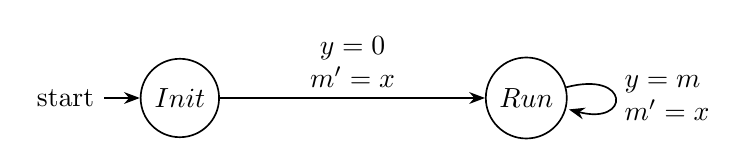
\begin{tikzpicture}[>=Stealth,auto,node distance=4.4cm,semithick]
  \node[state,initial] (init) {$Init$};
  \node[state,right of=init] (run) {$Run$};
  \path[->]
    (init) edge node[midway,above,align=center]
      {$y = 0$\\$m' = x$} (run)
    (run) edge[loop right] node[align=left]
      {$y = m$\\$m' = x$} (run);
\end{tikzpicture}
\caption{Program automaton for \texttt{delay\_int}.}
\end{figure}

If \(u = (u_0,u_1,u_2,\dots)\), the stream semantics yields:
\[
y_0 = 0,
\qquad
y_{k+1} = u_k.
\]
That is,
\[
y = (0,u_0,u_1,u_2,\dots).
\]

\subsection{Example: \texttt{toggle}}

The \texttt{toggle} example alternates the output between \(0\) and \(1\). It
can be represented with a Boolean memory state \(m \in \{0,1\}\):
\begin{align*}
\StepRel(t_{init},Init,m,\star,Run,m',y)
&:\Longleftrightarrow
y = 0 \land m' = 1,\\
\StepRel(t_{run},Run,m,\star,Run,m',y)
&:\Longleftrightarrow
y = m \land m' = 1 - m.
\end{align*}

\begin{figure}[h]
\centering
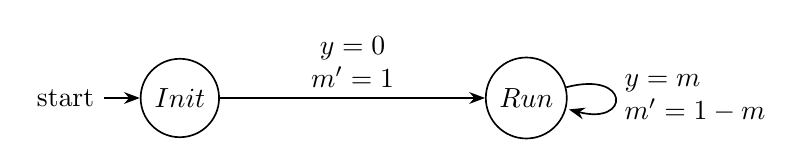
\begin{tikzpicture}[>=Stealth,auto,node distance=4.4cm,semithick]
  \node[state,initial] (init) {$Init$};
  \node[state,right of=init] (run) {$Run$};
  \path[->]
    (init) edge node[midway,above,align=center]
      {$y = 0$\\$m' = 1$} (run)
    (run) edge[loop right] node[align=left]
      {$y = m$\\$m' = 1-m$} (run);
\end{tikzpicture}
\caption{Program automaton for \texttt{toggle}.}
\end{figure}

\section{Specification, Observations, and Guarantees}

\subsection{From Alphabet Words to Semantic Observations}

Automaton labels do not necessarily range over a finite syntactic alphabet.
They may instead be read as predicates over semantic observations.

\begin{definition}[Observation Domains]
In Kairos, one uses in practice:
\begin{itemize}[leftmargin=1.4em]
\item \(X_A = I\) for the assumption automaton \(A\);
\item \(X_G = I \times O\) for the guarantee automaton \(G\);
\item more generally, a tick context derived from the trace if labels mention
  history.
\end{itemize}
\end{definition}

\begin{remark}
The presence of past atoms such as \(prev(x)\) does not change the nature of
the automaton. It only means that the label is evaluated on the trace through a
local context \(\ctx_u(k)\) rich enough to interpret the past. In the
implementation, this reading is then compiled through finite auxiliary
variables; these variables are not part of the source semantics.
\end{remark}

\subsection{Guarantee Examples}

For \texttt{delay\_int}, the guarantee is
\[
X\,G(y = prev(x)).
\]
The compiled automaton is a finite residual automaton, not an automaton
parameterized by an implicit value. We therefore use three states:
\[
Mon_0,\qquad Mon_1,\qquad Mon_{bad}.
\]

\begin{figure}[h]
\centering
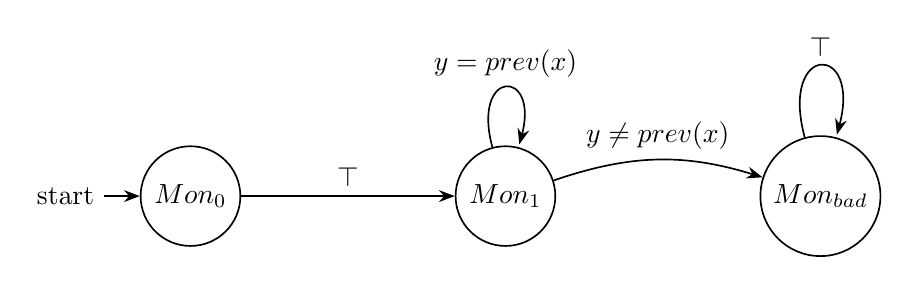
\begin{tikzpicture}[>=Stealth,auto,node distance=4.0cm,semithick]
  \node[state,initial] (m0) {$Mon_0$};
  \node[state,right of=m0] (m1) {$Mon_1$};
  \node[state,right of=m1] (mb) {$Mon_{bad}$};
  \path[->]
    (m0) edge node[midway,above] {$\top$} (m1)
    (m1) edge[loop above] node {$y = prev(x)$} (m1)
    (m1) edge[bend left=18] node[midway,above] {$y \neq prev(x)$} (mb)
    (mb) edge[loop above] node {$\top$} (mb);
\end{tikzpicture}
\caption{Guarantee automaton for \texttt{delay\_int}.}
\end{figure}

For \texttt{toggle}, the guarantee expects alternation \(0,1,0,1,\dots\):

\begin{figure}[h]
\centering
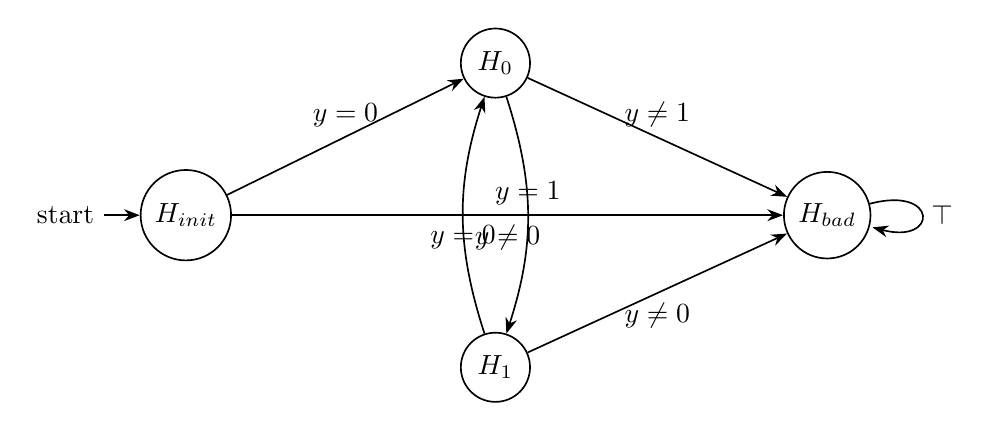
\begin{tikzpicture}[>=Stealth,auto,node distance=4.0cm,semithick]
  \node[state,initial] (q0) {$H_{init}$};
  \node[state,above right=1.2cm and 3.2cm of q0] (qz) {$H_0$};
  \node[state,below right=1.2cm and 3.2cm of q0] (qo) {$H_1$};
  \node[state,right=7.0cm of q0] (qb) {$H_{bad}$};
  \path[->]
    (q0) edge node[midway,above] {$y = 0$} (qz)
    (q0) edge node[midway,below] {$y \neq 0$} (qb)
    (qz) edge[bend left=18] node[midway,above] {$y = 1$} (qo)
    (qo) edge[bend left=18] node[midway,below] {$y = 0$} (qz)
    (qz) edge node[midway,above] {$y \neq 1$} (qb)
    (qo) edge node[midway,below] {$y \neq 0$} (qb)
    (qb) edge[loop right] node {$\top$} (qb);
\end{tikzpicture}
\caption{Guarantee automaton for \texttt{toggle}.}
\end{figure}

\section{Explicit Product \texorpdfstring{\(program \times A \times G\)}{program x A x G}}

\subsection{Intuition}

The explicit product is not meant to artificially ``glue together'' three
graphs. It represents the following semantic fact: at each tick \(k\),
\begin{enumerate}[leftmargin=1.4em]
\item the program reads \(i(k)\) and produces \(o(k)\);
\item \(A\) reads \(i(k)\);
\item \(G\) reads \((i(k),o(k))\).
\end{enumerate}
There is therefore a \emph{unique synchronized step} of the product.

\subsection{Product States and Steps}

\begin{definition}[Program State and Product State]
We write
\[
\mathsf{PState} := S.
\]
A product state is a triple
\[
\mathsf{ProdState} := S \times Q_A \times Q_G.
\]
\end{definition}

\begin{remark}
This is indeed the \emph{finite} component of the product. Memory, input, and
output do not belong to the product state in the current Rocq formalization;
they appear at the level of the concrete step and the local context.
\end{remark}

\begin{definition}[Product Run]
For an input stream \(u\), we define:
\[
\rps(u,k) :=
\bigl(s_u(k),\, q_A(k),\, q_G(k)\bigr),
\]
where \(q_A\) is the run of \(A\) on \(u\), and \(q_G\) is the run of \(G\) on
\(\run(u)\).
\end{definition}

\begin{definition}[Product Step]
A product step \(p\) is an object of the form
\[
p = \bigl((s,q_A,q_G),\, m,\, i,\, t,\, e_A,\, e_G \bigr)
\]
such that:
\begin{enumerate}[leftmargin=1.4em]
\item the concrete program step satisfies
  \[
  ((s,m),i)\xrightarrow{\,t\,}_P((s',m'),o);
  \]
\item \(\mathsf{src}_A(e_A)=q_A\) and \(\mathsf{Lab}_A(e_A)(i)=\True\) and
  \(\mathsf{dst}_A(e_A)=q_A'\);
\item \(\mathsf{src}_G(e_G)=q_G\) and \(\mathsf{Lab}_G(e_G)(i,o)=\True\) and
  \(\mathsf{dst}_G(e_G)=q_G'\).
\end{enumerate}
\[
\text{The target of the step is then } (s',q_A',q_G').
\]
\end{definition}

\begin{remark}
The first point of this definition can also be read as
\[
((s,m),i)\xrightarrow{\,t\,}_P((s',m'),o),
\]
which makes the synchronization between the program step, the reading of \(A\)
on \(i\), and the reading of \(G\) on \((i,o)\) more visible, without making
memory part of the finite product state.
\end{remark}

\begin{remark}
Everything is written here as a logical relation:
\[
\StepRel(t,s,m,i,s',m',o),
\qquad
\mathsf{Lab}_A(e_A)(i),
\qquad
\mathsf{Lab}_G(e_G)(i,o).
\]
We deliberately avoid imperative notations such as \(m := i\), which suit the
code but not the mathematical model.
\end{remark}

\subsection{Why This Product Is the Right Object}

The explicit product plays three roles.
\begin{enumerate}[leftmargin=1.4em]
\item It gives a common semantics to the program and the automata.
\item It makes it possible to talk locally about situations in which \(G\) is
  about to be violated.
\item It provides a unique basis for the Rocq proof and for the product IR in
  the current implementation.
\end{enumerate}

In particular, the product explains why a concrete tick is always described by a
minimal quadruple of information:
\[
\text{product source},\qquad \text{input},\qquad \text{output},\qquad \text{product target}.
\]

\subsection{Example: Relevant Subgraph of \texttt{delay\_int}}

In \texttt{delay\_int}, the relevant product states are:
\[
\bigl(Init,A_{ok},Mon_0\bigr),
\qquad
\bigl(Run,A_{ok},Mon_1\bigr),
\qquad
\bigl(Run,A_{ok},Mon_{bad}\bigr).
\]
The first tick goes from \(Mon_0\) to \(Mon_1\). Afterwards, the only step that
really matters for correctness is the one that would go to \(Mon_{bad}\).

\begin{figure}[h]
\centering
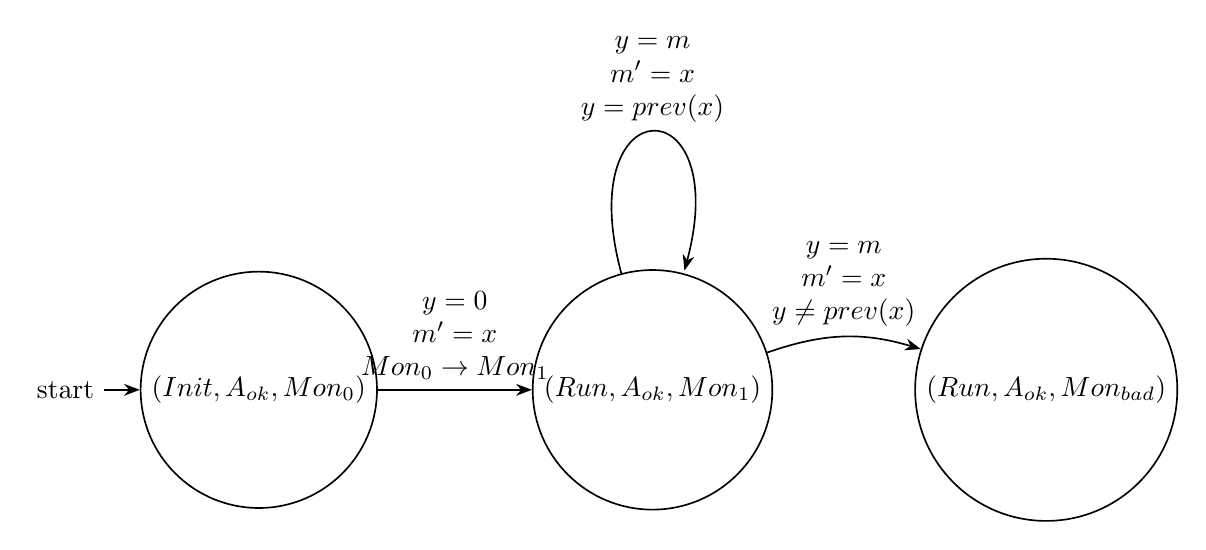
\begin{tikzpicture}[>=Stealth,auto,node distance=5.0cm,semithick]
  \node[state,initial] (p0) {$(Init,A_{ok},Mon_0)$};
  \node[state,right of=p0] (p1) {$(Run,A_{ok},Mon_1)$};
  \node[state,right of=p1] (pb) {$(Run,A_{ok},Mon_{bad})$};
  \path[->]
    (p0) edge node[midway,above,align=center]
      {$y=0$\\$m'=x$\\$Mon_0 \to Mon_1$} (p1)
    (p1) edge[loop above] node[align=center]
      {$y=m$\\$m'=x$\\$y = prev(x)$} (p1)
    (p1) edge[bend left=18] node[midway,above,align=center]
      {$y=m$\\$m'=x$\\$y \neq prev(x)$} (pb);
\end{tikzpicture}
\caption{Relevant product subgraph for \texttt{delay\_int}.}
\end{figure}

\section{Dangerous Steps and Local Obligations}

\subsection{Dangerous Step}

The central notion of Kairos is now easy to define.

\begin{definition}[Dangerous Step]
A product step
\[
p :
\bigl(s,q_A,q_G\bigr)
\longrightarrow
\bigl(s',q_A',q_G'\bigr)
\]
is \emph{dangerous} if
\[
q_A' \neq bad_A
\qquad\text{and}\qquad
q_G' = bad_G.
\]
\end{definition}

\paragraph{Intuition.}
This is not just any step to a bad state. One must distinguish two cases:
\begin{itemize}[leftmargin=1.4em]
\item if \(A\) itself goes to \(bad_A\), then one leaves the admissible input
  domain; this is not the main objective of the conditional theorem;
\item if \(A\) remains admissible but \(G\) goes to \(bad_G\), then an
  admissible input is enough to produce a guarantee violation. This is the
  situation that must be ruled out locally.
\end{itemize}

\paragraph{Connection to the global semantics.}
If \(\AvoidG(\run(u))\) is false, there exists a first index \(k\) such that
\(q_G(k+1)=bad_G\). Tick \(k\) then realizes a dangerous step. This observation
is what allows one to move from a global violation over an infinite word to a
local witness at a single tick.

\subsection{Local Context and Matching Relation}

\paragraph{Why introduce a local context?}
Obligation generation is static: it ranges over abstract product steps. Actual
execution is dynamic: at each tick it realizes a concrete program transition and
advances \(A\) and \(G\). To connect these two levels, one must summarize the
concrete tick by a local object, and then state when this object realizes a
given abstract step.

\paragraph{Concrete tick versus abstract step.}
The \emph{concrete tick} at rank \(k\) is the step actually observed in an
execution under an input stream \(u\): current configuration, current input,
current output, and next configuration. The \emph{abstract product step} is a
purely static object, enumerated by the generator, which describes a possible
transition of the triple \(program \times A \times G\). Obligations are
generated over abstract steps and then validated over all concrete ticks.

\begin{definition}[Factored Local Context]
The local context of tick \(k\) under input \(u\) is
\[
\ctx(u,k):=
\bigl(\mathsf{src}_{u,k},\mathsf{obs}_{u,k},\mathsf{dst}_{u,k}\bigr),
\]
where
\begin{align*}
\mathsf{src}_{u,k} &:= \bigl(s_u(k),m_u(k),q_A(k),q_G(k)\bigr),\\
\mathsf{obs}_{u,k} &:= \bigl(u(k),o_u(k)\bigr),\\
\mathsf{dst}_{u,k} &:= \bigl(s_u(k+1),m_u(k+1),q_A(k+1),q_G(k+1)\bigr).
\end{align*}
\end{definition}

\begin{remark}
This factorization replaces a hard-to-read 10-tuple with three named blocks:
local source, local observation, and local target. It also matches the right
intuition of the underlying Rocq structure: \texttt{StepCtx} carries the
concrete tick, and \texttt{product\_step\_realizes\_at} relates this tick to an
abstract step.
\end{remark}

\begin{definition}[Matching a Step]
Let
\[
p = \bigl((s,q_A,q_G),m,i,t,e_A,e_G\bigr)
\]
be an abstract product step. We say that
\(\ctx=(\mathsf{src},\mathsf{obs},\mathsf{dst})\) \emph{realizes} \(p\), and we
write \(\Match(\ctx,p)\), if:
\begin{enumerate}[leftmargin=1.4em]
\item \(\mathsf{src} = (s,m,q_A,q_G)\);
\item \(\mathsf{obs} = (i,o)\) for some output \(o\);
\item the program step is indeed
  \[
  ((s,m),i)\xrightarrow{\,t\,}_P((s',m'),o);
  \]
\item edge \(e_A\) moves \(A\) from \(q_A\) to \(q_A'\) on \(i\);
\item edge \(e_G\) moves \(G\) from \(q_G\) to \(q_G'\) on \((i,o)\);
\item \(\mathsf{dst} = (s',m',q_A',q_G')\).
\end{enumerate}
\end{definition}

\begin{remark}
In Rocq, the primitive relation \texttt{ctx\_matches\_ps} is intentionally more
minimal: it only looks at the current state, the current memory, the current
input, and the selected program transition. The well-formedness of the step
(\texttt{product\_step\_wf}) and its realization
(\texttt{product\_step\_realizes\_at}) then reconstruct the correct automaton
target. The paper develops the full intuition of this matching while remaining
faithful to that decomposition.
\end{remark}

\subsection{Obligation Associated with a Dangerous Step}

\begin{definition}[Elementary Obligation]
To every dangerous product step \(p\), we associate the local formula
\[
\mathsf{obl}_p(\ctx) := \neg \Match(\ctx,p).
\]
\end{definition}

This form explains the exact intuition of the clause:
\begin{quote}
``at the current tick, it is impossible to simultaneously realize the chosen
program transition, the chosen assumption edge, and the guarantee edge leading
to \(bad_G\)''.
\end{quote}

\subsection{Detailed Example: \texttt{delay\_int}}

\paragraph{What Is Static.}
The generator first explores a product subgraph. For \texttt{delay\_int}, it
retains in particular the state
\[
(Run,A_{ok},Mon_1),
\]
and then the abstract steps leaving this state. Among them, only one is
dangerous: the one that keeps \(A\) in \(A_{ok}\) but takes \(G\) to
\(Mon_{bad}\).

In \texttt{delay\_int}, the dangerous step starts from
\[
(Run,A_{ok},Mon_1)
\]
and follows:
\begin{itemize}[leftmargin=1.4em]
\item the program transition \(t_{run}\), characterized by
  \[
  y = m \land m' = x;
  \]
\item the trivial edge of \(A\), always true;
\item the guarantee edge
  \[
  Mon_1 \xrightarrow{\, y \neq prev(x) \,} Mon_{bad}.
  \]
\end{itemize}

The clause generated from this step is
\[
\mathsf{obl}_{delay}(\ctx) := \neg \Match(\ctx,p_{delay}^{bad}).
\]
It is introduced because a concrete tick matching this step would move the
guarantee to \(Mon_{bad}\) while remaining admissible for \(A\).

Unfolding the matching yields, at the core of the clause, the conjunction
\[
o = m
\;\land\;
m' = x
\;\land\;
o \neq prev(x).
\]
Under the user invariant
\[
\UserInv(Run)(\ctx) : m = prev(x),
\]
this core becomes
\[
o = prev(x)
\;\land\;
o \neq prev(x),
\]
which is contradictory. The local clause therefore plays a very concrete
role: it prevents exactly the transition from \((Run,A_{ok},Mon_1)\) to
\((Run,A_{ok},Mon_{bad})\).

\subsection{Detailed Example: \texttt{toggle}}

In \texttt{toggle}, there are two families of dangerous steps:
\begin{itemize}[leftmargin=1.4em]
\item from guarantee state \(H_0\), every step producing \(y \neq 1\);
\item from guarantee state \(H_1\), every step producing \(y \neq 0\).
\end{itemize}

\begin{figure}[h]
\centering
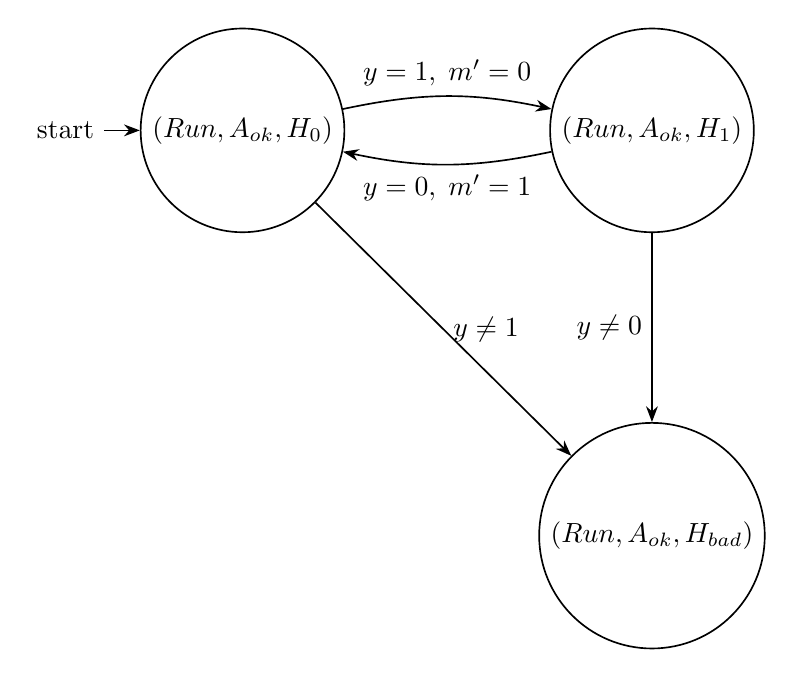
\begin{tikzpicture}[>=Stealth,auto,node distance=5.2cm,semithick]
  \node[state,initial] (h0) {$(Run,A_{ok},H_0)$};
  \node[state,right of=h0] (h1) {$(Run,A_{ok},H_1)$};
  \node[state,below=2.4cm of h1] (hb) {$(Run,A_{ok},H_{bad})$};
  \path[->]
    (h0) edge[bend left=12] node[midway,above]
      {$y = 1,\; m' = 0$} (h1)
    (h1) edge[bend left=12] node[midway,below]
      {$y = 0,\; m' = 1$} (h0)
    (h0) edge node[midway,right] {$y \neq 1$} (hb)
    (h1) edge node[midway,left] {$y \neq 0$} (hb);
\end{tikzpicture}
\caption{Safe and dangerous steps in the product of \texttt{toggle}.}
\end{figure}

Here again, the useful information does not come from a global temporal
formula, but from a subgraph of the product. Each local safety clause expresses
the negation of one of the matchings leading to \(H_{bad}\).

\section{Pseudo-Algorithmic Generation of Clauses and Triples}

\subsection{Why a Procedural Description Is Necessary}

It is not enough to enumerate clause families. To understand the Kairos
architecture, one must explain how the tool constructs them from the product.
The right view is the following:
\begin{enumerate}[leftmargin=1.4em]
\item explore reachable product states;
\item enumerate locally realizable product steps;
\item classify each step;
\item generate, according to this class, the appropriate clauses.
\end{enumerate}

\paragraph{Immediate Instantiation on \texttt{delay\_int}.}
This procedure already yields something very concrete:
\begin{enumerate}[leftmargin=1.4em]
\item the relevant reachable states are
  \[
  (Init,A_{ok},Mon_0)
  \quad\text{and}\quad
  (Run,A_{ok},Mon_1);
  \]
\item from \((Run,A_{ok},Mon_1)\), one enumerates one safe step and one
  dangerous step;
\item the dangerous step is classified as ``objective no bad'';
\item one adds the local safety clause
  \[
  \mathsf{obl}_{delay}(\ctx) = \neg \Match(\ctx,p_{delay}^{bad}).
  \]
\end{enumerate}
The general procedural view is therefore not an extra layer: it describes
exactly what the minimal \texttt{delay\_int} case already does.

\subsection{General Scheme}

\paragraph{Input.}
The generator receives:
\begin{itemize}[leftmargin=1.4em]
\item a program \(P\);
\item a specification \(\Phi = (A,G,\UserInv)\).
\end{itemize}

\paragraph{Output.}
It produces a set of semantic clauses, each equipped with:
\begin{itemize}[leftmargin=1.4em]
\item an abstract origin;
\item a state or step of the product;
\item a future backend projection.
\end{itemize}

\subsection{Conceptual Algorithm}

\begin{quote}
\textbf{For each} reachable product state \(x=(s,q_A,q_G)\):

\quad 1. Add the initial/coherence clauses attached to \(x\).

\quad 2. Add the user-invariant propagation clauses attached to \(x\), for example
\[
\mathsf{InvObl}_x(\ctx) :=
\bigl(\mathsf{src\_state}(\ctx)=s \land \mathsf{src\_a}(\ctx)=q_A \land \mathsf{src\_g}(\ctx)=q_G\bigr)
\Rightarrow
\bigl(\UserInv(s)(\ctx)\Rightarrow \mathsf{Shift}(\UserInv(s'))(\ctx)\bigr).
\]

\quad 3. Add the automaton-support clauses attached to
\quad \;\;\; \(x\), that is, the formulas that justify the additional local
\quad \;\;\; automaton facts assumed by the backend.

\quad 4. \textbf{For each} product step \(p\) outgoing from \(x\):

\qquad a. If the target of \(p\) falls into \(bad_A\), only add the support
\qquad\;\;\; clauses that are still required.

\qquad b. If \(p\) is dangerous, add the objective clause
\[
\mathsf{ObjObl}_p(\ctx) := \neg \Match(\ctx,p).
\]

\qquad c. If \(p\) is safe, only add the coherence and support clauses
\qquad\;\;\; required for this step.
\end{quote}

\noindent
The point of this procedural presentation is that \emph{NoBad clauses are not
expected to be discharged in isolation}. The backend proves them inside
transition-level Hoare bundles, under extra local assumptions, and those
assumptions are themselves justified by generated helper clauses. The local
proof architecture therefore has one safety layer and one helper layer:
\begin{enumerate}[leftmargin=1.4em]
\item \(\mathsf{Helper/InitGoal}\): establish, at the initial tick, both the
  user-invariant facts and the automaton-support facts;
\item \(\mathsf{Helper/Propagation}\): propagate, from one tick to the next,
  both the user-invariant facts and the automaton-support facts;
\item \(\mathsf{Safety/NoBad}\): exclude dangerous product steps under this
  helper context.
\end{enumerate}

In the current Rocq core, this architecture is reconstructed in two steps.
First, the concrete generation relation produces semantic clauses. Second,
these clauses are assembled into relational Hoare triples whose validity is
stated against the relational semantics of program transitions. The concrete
generation relation contains:
\[
\mathsf{prod\_clause}(ps)(\ctx) := \neg \ctx\mathsf{\_matches\_ps}(\ctx,ps)
\]
for the objective layer, a preservation-style clause for node invariants, and a
preservation-style clause for automaton support. The Rocq kernel now turns such
clauses into relational Hoare triples; the implementation further groups these
triples by program transition before translating them to Why3-facing
verification tasks. What is still more fine-grained on the
implementation side is the internal distinction between monitor-compatibility
support and state-aware assumption support.

The implementation now exposes both levels explicitly:
\begin{itemize}[leftmargin=1.4em]
\item a four-way conceptual projection used to summarize generated clauses as
  \(\mathsf{NoBad}\), \(\mathsf{InitialGoal}\),
  \(\mathsf{UserInvariant}\), and \(\mathsf{AutomatonSupport}\);
\item a finer backend taxonomy that keeps separate OBC/Why3-facing families
  such as \texttt{FamNoBadRequires}, \texttt{FamNoBadEnsures},
  \texttt{FamInitialCoherencyGoal}, \texttt{FamCoherencyRequires},
  \texttt{FamCoherencyEnsuresShifted},
  \texttt{FamMonitorCompatibilityRequires}, and
  \texttt{FamStateAwareAssumptionRequires}.
\end{itemize}
The finer families are projected onto the same four conceptual categories as
the Rocq proof architecture. These four categories are a classification of
\emph{generated clauses}, not four independent proof phases.

\subsection{Four Obligation Categories}

The generated semantic clauses fall into four conceptual categories.

\paragraph{NoBad.}
These are the genuine safety objectives. For a dangerous product step \(p\), the
semantic clause is:
\[
\mathsf{NoBad}_p(\ctx) := \neg \Match(\ctx,p).
\]
The backend does not normally send this clause in isolation to the external
tool. The kernel first turns it into a relational Hoare triple whose
postcondition is \(\bot\) on the dangerous branch; the implementation then
places that triple inside a transition-level proof bundle together with the
helper preconditions and postconditions needed to make it provable.
These clauses are sufficient to conclude that the product never reaches
\(bad_G\), but they are not expected to be discharged without helper clauses.

\paragraph{InitialGoal.}
These clauses provide the base case of the induction. They establish that
the helper context already holds at tick \(0\). Concretely, this includes:
\begin{itemize}[leftmargin=1.4em]
\item initialization of the user invariant attached to the initial node;
\item initialization of the automaton-support facts attached to the initial
  product state.
\end{itemize}
In the implementation, they correspond to explicit initial helper triples grouped
in the same initial helper bundle. They could equivalently be encoded by a
ghost predecessor carrying \(\top\), but keeping them explicit is simpler and
clearer.

\paragraph{UserInvariant.}
These clauses justify the node invariants used as local preconditions. The
implementation injects:
\begin{itemize}[leftmargin=1.4em]
\item \(\mathsf{Inv}(\mathsf{src})\) in transition preconditions;
\item \(\mathsf{Shift}(\mathsf{Inv}(\mathsf{dst}))\) in transition
  postconditions.
\end{itemize}
So the predecessor proves the fact that the successor later consumes as
its own precondition. In the Rocq kernel this is expressed by a relational
Hoare triple whose postcondition talks about the successor context. This is one
\emph{subfamily} of the common helper propagation layer. These clauses must be
bundled together with automaton
support clauses for the same transition, because each side may help prove the
other.

\paragraph{AutomatonSupport.}
These clauses justify the automaton-derived facts added to transition
preconditions. There are two important subcases in the implementation:
\begin{itemize}[leftmargin=1.4em]
\item monitor compatibility clauses: if the current monitor state is \(q\),
  then one of the incoming guards leading to \(q\) must have held at the
  previous tick, after shifting;
\item state-aware assumption/product support clauses: for a fixed program
  transition and current guarantee state, one of the locally compatible
  \((A\text{-guard} \land G\text{-guard})\) disjuncts must hold.
\end{itemize}
This is the second \emph{subfamily} of the common helper propagation layer.
Again, in the Rocq kernel these clauses feed relational Hoare triples whose
postconditions speak about the successor context. They are not meant to live in
proof objects separate from user
invariants: they must be discharged in the same helper bundles.

Transition-level user contracts remain visible in the backend as separate
\texttt{transition\_requires} and \texttt{transition\_ensures} families, but
they do not belong to the four generated-proof categories above. They are part
of the user specification surface, not clauses generated by the local
product proof architecture itself.

\paragraph{Why the helper/safety split is needed.}
The soundness point is the following:
\begin{quote}
it is valid to enrich a local dangerous-step proof with additional
preconditions only if generated clauses separately establish that these
preconditions do hold on concrete executions.
\end{quote}
Therefore:
\begin{enumerate}[leftmargin=1.4em]
\item \(\mathsf{Helper/InitGoal}\) provides the base case for both invariant
  facts and automaton-support facts;
\item \(\mathsf{Helper/Propagation}\) propagates both kinds of helper facts
  through time, inside the same transition-level proof objects;
\item \(\mathsf{Safety/NoBad}\) excludes the dangerous product steps under this
  common helper context.
\end{enumerate}

\begin{remark}
The four labels
\(\mathsf{NoBad}\), \(\mathsf{InitialGoal}\), \(\mathsf{UserInvariant}\), and
\(\mathsf{AutomatonSupport}\) are useful as a classification of generated
clauses. However, the proof architecture is not a chain of four isolated
layers: \(\mathsf{UserInvariant}\) and \(\mathsf{AutomatonSupport}\) must be
bundled together inside the same helper proof objects, both at initialization
and at propagation time.
\end{remark}

\section{Proof Structure}

\subsection{Internal and External Hypotheses}

The proof structure mixes two levels that must be separated explicitly.

\paragraph{Internal hypotheses of the core.}
They belong to the Rocq modeling of the system:
\begin{itemize}[leftmargin=1.4em]
\item determinism of program steps and automaton selections;
\item non-badness of the initial states of \(A\) and \(G\);
\item well-formedness of realized product steps;
\item correctness of the shift operator used to transport delayed facts from one
  tick to the next.
\end{itemize}

\paragraph{External hypotheses.}
They concern the external validator:
\begin{itemize}[leftmargin=1.4em]
\item completeness of the external checker over the generated relational Hoare
  triples (or over the transition-level bundles obtained by grouping them);
\item soundness of triple or bundle validation, that is, validity of the
  generated semantic clauses covered by successful proof objects.
\end{itemize}

The final theorem uses the external hypotheses only at the last step of the
proof; the rest of the reduction is proved inside the core.

\subsection{From Global Violation to Dangerous Step}

\begin{lemma}[First Violating Tick]
For every input stream \(u\), if \(\neg \AvoidG(\run(u))\), then there exists an
index \(j\) such that \(q_G(j)=bad_G\). Since the initial state of \(G\) is not
bad, one must have \(j=S\,k\) for some \(k\).
\end{lemma}

\begin{proof}[Proof sketch]
One unfolds the negation of \(\AvoidG\). The Rocq formalization uses a
classical step to obtain the existence of a bad index, and then the hypothesis
\texttt{G\_init\_not\_bad} to exclude the initial case.
\end{proof}

\begin{lemma}[Global Violation Implies Dangerous Step]
For every input stream \(u\), if \(\AvoidA(u)\) and \(\neg \AvoidG(\run(u))\),
then there exists a tick \(k\) such that \(bad\_local\_step(u,k)\).
\end{lemma}

\begin{proof}[Proof sketch]
This is exactly theorem \texttt{bad\_local\_step\_if\_G\_violated} in the Rocq
formalization. The constructed dangerous step is a
\texttt{product\_select\_at u k}, well-formed and realized at tick \(k\), whose
target keeps \(A\) out of \(bad_A\) and places \(G\) in \(bad_G\).
\end{proof}

\subsection{From Dangerous Step to Local Obligation}

\begin{lemma}[Validity of Helper Triples]
For every well-formed product step \(ps\), the helper information needed for
the successor tick is propagated by generated relational Hoare triples attached
to the underlying program transition of \(ps\).
\end{lemma}

\begin{proof}[Proof sketch]
The current kernel proves two inductive propagation lemmas:
\texttt{node\_inv\_holds\_on\_run} and
\texttt{support\_automaton\_holds\_on\_run}. Their proofs no longer assume the
invariant globally. Instead, they use:
\begin{itemize}[leftmargin=1.4em]
\item an initial helper triple for the base case;
\item a propagation helper triple for each realized product step;
\item validity of the generated helper triples.
\end{itemize}
\end{proof}

\begin{lemma}[Local Coverage]
For every input stream \(u\) and every tick \(k\), if \(bad\_local\_step(u,k)\),
then there exists a generated semantic clause \(obl\) such that:
\[
Generated(obl)
\qquad\text{and}\qquad
\neg obl(\ctx(u,k)).
\]
\end{lemma}

\begin{proof}[Proof sketch]
The theorem \texttt{generation\_coverage} selects the canonical clause
\texttt{prod\_clause ps} produced from the realized dangerous step \(ps\).
Since \texttt{ctx\_at\_matches\_realized\_ps} shows that the current context
matches this step, the clause \(\neg \Match\) is indeed violated at the
considered tick.
\end{proof}

\subsection{Conditional Correctness Theorem}

\begin{theorem}[Conditional Correctness]
Assume the following validity hypothesis:
\begin{enumerate}[leftmargin=1.4em]
\item \emph{validity of generated triples}:
  \[
  \forall ht,\; GeneratedTriple(ht) \Rightarrow TripleValid(ht).
  \]
\end{enumerate}
Then, for every input stream \(u\),
\[
\AvoidA(u) \Rightarrow \AvoidG(\run(u)).
\]
\end{theorem}

\begin{proof}
Fix an input stream \(u\) and assume \(\AvoidA(u)\). Suppose, for contradiction,
\(\neg \AvoidG(\run(u))\). The previous lemma then yields a tick \(k\) and a
generated triple \(ht\) such that \texttt{GeneratedTriple(ht)}, the
precondition of \(ht\) holds on \(\ctx(u,k)\), and \(ht\) is exactly the
\texttt{no\_bad\_triple} attached to the realized dangerous step. By validity
of generated triples, \(ht\) is valid. Applying this valid triple to the
realized transition contradicts the fact that its postcondition is
\(\False\).
\end{proof}

\section{Implementation Language and Why3 Backend}

\subsection{Source Language of the Implementation}

The mathematical model introduced above is reflected in the current Kairos
implementation through two layers that are kept conceptually distinct.

\paragraph{Program layer.}
A node contains:
\begin{itemize}[leftmargin=1.4em]
\item input and output declarations;
\item local variables and state variables;
\item a finite set of control states and an initial control state;
\item a transition relation described by guarded node transitions.
\end{itemize}
This is the executable part of the source program.

\paragraph{Specification layer.}
The same node carries:
\begin{itemize}[leftmargin=1.4em]
\item assumptions, interpreted over input traces;
\item guarantees, interpreted over reactive input/output traces;
\item state-related user invariants, interpreted over local trace contexts.
\end{itemize}
In the implementation, this split is explicit: the program part provides the
transition semantics, while the specification part provides the formulas from
which automata and support clauses are derived.

\subsection{From Detailed Clauses to Backend Code}

The detailed semantic clauses defined in this paper are not sent to Why3 as raw
\(\neg \Match(\ctx,p)\) formulas over abstract product steps. They are first
assembled into relational Hoare triples and then projected to a finite backend
representation.

\paragraph{Step 1: product analysis.}
The implementation builds or explores the product
\(program \times A \times G\). This exploration computes:
\begin{itemize}[leftmargin=1.4em]
\item reachable product states;
\item realizable product steps;
\item the classification of steps into safe, dangerous, inadmissible, or
  pruned;
\item the abstract local clauses attached to those states and steps.
\end{itemize}

\paragraph{Step 2: backend projection.}
These abstract clauses and triples are then compiled into an instrumented
program:
\begin{itemize}[leftmargin=1.4em]
\item automaton information is represented by finite backend variables such as
  \texttt{\_\_aut\_state};
\item references to past values are compiled through auxiliary variables such
  as \texttt{\_\_pre\_k\ldots};
\item local clauses become backend preconditions, postconditions, linking
  invariants, and transition-side formulas.
\end{itemize}
The purpose of this projection is not to change the semantics, but to replace
the explicit matching relation over product steps with formulas that Why3 can
attach to concrete program declarations.

\paragraph{Step 3: Why3 generation.}
From this instrumented intermediate form, Kairos produces:
\begin{itemize}[leftmargin=1.4em]
\item an OBC-like textual form used for debugging and inspection;
\item a Why3 abstract syntax tree;
\item a rendered Why3 source file;
\item optional verification-condition and SMT dumps, one block per goal.
\end{itemize}
At this stage, the triples of the paper have become Why3 verification
conditions attached to functions, transitions, and auxiliary lemmas of the
generated program.

\subsection{What Is Actually Sent to Why3}

The object sent to Why3 is therefore not the mathematical product itself, but a
finite program annotated with the formulas that result from the projection
above. Concretely, the generated Why3 file contains:
\begin{itemize}[leftmargin=1.4em]
\item declarations for program states, memories, and auxiliary variables;
\item one or more Why3 procedures encoding the program step relation;
\item preconditions and postconditions representing the projected clauses;
\item additional formulas linking source variables, target variables, automaton
  states, and history variables.
\end{itemize}

From the point of view of the present paper, the essential invariant is the
following: every backend verification condition must correspond to a semantic
fact justified by the product analysis. In particular, dangerous product steps
must give rise to formulas whose failure would exactly witness the local
realization of such a step.

\paragraph{Additional structural side conditions.}
Because the abstract model assumes that every tick computes a successor state,
a successor memory, and an output valuation, a practical Kairos backend may
need companion checks or side conditions ensuring that the concrete program
falls within this fragment. Such conditions concern, for instance, the absence
of runtime blocking caused by invalid operations, the fact that each output
signal is assigned a value at every instant, and the exhaustiveness of the
transition filtering by current state and memory. These conditions do not
belong to the abstract product core itself; they are prerequisites for applying
the abstract semantics to the concrete source language.

\subsection{What Kairos Retrieves from Why3}

When Why3 is invoked, Kairos receives a collection of proof goals together with
their statuses. For each goal, the relevant result is one of the standard Why3
outcomes: proved, invalid, unknown, timeout, or backend failure.

\paragraph{Meaning of a positive result.}
If a goal is proved, then the corresponding projected backend formula is valid
in the logic handled by Why3 and its external provers. Under the intended
correctness theorem of the paper, such a result is used as evidence that the
associated local triple is valid, and therefore that its underlying clause or
support condition holds. This also applies to
any side conditions or companion checks used to guarantee that the concrete
program belongs to the total fragment assumed by the model.

\paragraph{Meaning of a negative or inconclusive result.}
If a goal is reported invalid, unknown, timed out, or failed, the mathematical
meaning is weaker than ``the property is false''. It means that Kairos did not
obtain external validation for the projected formula. This may reveal:
\begin{itemize}[leftmargin=1.4em]
\item a real bug in the program or in the specification;
\item an insufficient invariant or support clause;
\item a weakness of the backend encoding;
\item or a limitation of the automatic prover.
\end{itemize}
Hence the result returned by Why3 must always be interpreted relative to the
projection correctness assumptions of the overall method.

\subsection{Why the Backend Still Matters}

The explicit product remains the right semantic reference, but it is not the
right final object to materialize exhaustively in generated Why3 code. The
backend remains necessary in order to:
\begin{itemize}[leftmargin=1.4em]
\item keep the generated code finite and manageable;
\item encode automaton and history information through ordinary program
  variables;
\item expose triples and their projected clauses in a format accepted by Why3 and SMT solvers.
\end{itemize}
The methodological split is therefore the following:
\begin{itemize}[leftmargin=1.4em]
\item the product provides the semantic source of the clauses;
\item the backend packages them into transition-level triples and provides
  their finite proof-oriented encoding.
\end{itemize}

\section{Related Work}

The closest related work falls into two broad families. The first one studies
the verification of temporal properties of programs by compiling those
properties into automata or annotations that are then discharged by a program
verification backend. The second one studies synchronous or contract-based
verification frameworks in which assumptions, guarantees, observers, or
realizability checks play a central role. Kairos is closest to the first family
from the viewpoint of proof objects, and to the second from the viewpoint
of reactive assume/guarantee semantics.

\subsection{From Temporal Properties to Program Proof Objects}

\paragraph{Aorai.}
Aorai~\cite{aorai-manual,stouls-groslambert-2009} is probably the closest
neighbor to Kairos if one focuses on the idea of compiling temporal properties
into local proof material attached to a program. In Aorai, LTL properties about
C programs are translated into automata and then into ACSL-style annotations
checked by the Frama-C toolchain. The key similarity with Kairos is the
reduction from a global temporal property to finitely many local proof
objects. The main difference is semantic. Aorai is centered on annotated C
programs and temporal properties over program traces, whereas Kairos is
centered on reactive traces with an explicit distinction between input
assumptions and input/output guarantees. Kairos also makes the product
\(program \times A \times G\) explicit as a semantic object, instead of keeping
the automaton/program synchronization mostly implicit in the generated
annotations.

\paragraph{CaFE.}
CaFE~\cite{cafe-page} extends the same general ecosystem to CaRet properties,
which are tailored to nested calls and returns. This makes it especially
relevant when temporal reasoning must account for call-stack structure. Its
proximity to Kairos lies in the idea that temporal reasoning over programs can
be reduced to local proof objects checked by an existing backend. Its
difference from Kairos lies in the observed semantic domain: CaFE is organized
around call/return structure of C executions, whereas Kairos is organized
around reactive ticks, stateful stream semantics, and assume/guarantee safety on
input/output traces.

\subsection{Assume/Guarantee and Synchronous Verification}

\paragraph{AGREE.}
AGREE~\cite{agree-techreport,agree-observers} is close to Kairos on the logical
structure of specifications. It emphasizes assumptions and guarantees attached
to components, and it supports observer-style encodings of temporal patterns.
This places it closer to Kairos than Aorai with respect to contract structure.
However, AGREE works at an architectural and compositional level, not at the
level of an explicit semantic product between a program automaton and two
safety automata. Kairos differs by making the local product step itself the
primary justification point for local clauses.

\paragraph{Kind 2 and CoCoSpec.}
Kind~2~\cite{kind2-realizability} and CoCoSpec~\cite{cocospec} are also strong
reference points for contract-based reasoning on synchronous systems. Kind~2
offers realizability checking and proof support for Lustre-style programs and
contracts, while CoCoSpec provides a mode-aware contract language for reactive
systems. These systems are close to Kairos in their emphasis on reactive
contracts and explicit assumptions/guarantees. The main difference is again the
central semantic object. Kairos builds its local proof story around the product
between a program, an assumption automaton, and a guarantee automaton. Kind~2
and CoCoSpec are closer to invariant generation, model checking, and contract
reasoning directly over synchronous transition systems than to an explicit local
matching relation between concrete ticks and abstract product steps.

\paragraph{Lustre and theorem proving.}
Older work on Lustre and theorem proving~\cite{lustre-pvs} is also relevant as
historical background. It already combines a reactive programming language with
machine-checked reasoning and therefore shares with Kairos the ambition of
giving a mathematical semantics that supports actual proofs. Kairos differs by
organizing the reduction around safety automata and locally generated
clauses and triples, rather than around direct theorem proving over the source
transition system alone.

\subsection{Monitoring and Observer Compilation}

\paragraph{Copilot.}
Copilot~\cite{copilot-github,copilot3} is an important point of comparison on
the compilation side. It compiles temporal and stream-oriented specifications
into executable monitors, typically generating hard real-time C code. This is
close to Kairos in the sense that both approaches turn temporal specifications
into finite operational artifacts. The main difference is that Copilot is first
and foremost a runtime verification framework, whereas Kairos uses its compiled
artifacts to generate proof objects for deductive verification. Thus,
artifacts to generate deductive proof objects. Thus,
Copilot is particularly relevant as related work on monitor compilation, but it
is further from Kairos than Aorai, AGREE, or Kind~2 on the proof-theoretic
side.

\subsection{Position of Kairos}

Relative to these systems, Kairos combines four ingredients that are rarely
present together in a single framework:
\begin{itemize}[leftmargin=1.4em]
\item a reactive program semantics on streams;
\item an explicit input assumption automaton and an explicit guarantee
  automaton;
\item a semantic product \(program \times A \times G\) used as the source of
  local clauses;
\item a proof-oriented reduction from global bad executions to falsified local
  safety clauses and invalidated triples.
\end{itemize}
This makes Kairos simultaneously close to annotation-based temporal program
verification, to assume/guarantee reasoning for synchronous systems, and to the
observer-compilation tradition, while remaining distinct from each of these
families in the role played by the explicit product.

\section{Discussion}

\subsection{Why One Must Constantly Return to the Product}

A major source of confusion in this kind of document is to talk about
clauses as if they were floating formulas. In reality, every Kairos
clause must always be read as the projection of some information carried by
the product:
\begin{itemize}[leftmargin=1.4em]
\item a reachable product state;
\item a safe product step;
\item a dangerous product step;
\item or a user annotation reattached to that state or step.
\end{itemize}
This discipline explains the editorial choice of the present text: it returns
systematically to the program and to the product before discussing the backend.

\subsection{Limits of the Present Note}

This document does not claim to replace:
\begin{itemize}[leftmargin=1.4em]
\item the detailed Rocq proof;
\item the exhaustive description of the Why3/OBC backend;
\item or a complete complexity study.
\end{itemize}
Its aim is more focused: to provide a mathematical presentation that is complete
and pedagogical enough to serve as a stable reference between the proof, the
code, and the documentation.

\section{Conclusion}

The right central object for Kairos is the explicit product
\[
\text{program} \times A \times G.
\]
It makes the following simultaneously visible:
\begin{itemize}[leftmargin=1.4em]
\item the reactive semantics of the program on streams;
\item the reading of assumptions and guarantees by safety automata;
\item the notion of dangerous step;
\item the generation of local clauses and triples;
\item and the bridge both to the Rocq proof and to the external backend.
\end{itemize}

This refocusing has a simple methodological consequence: in a high-quality
article on Kairos, clauses must never be introduced as a mere list. They
must always appear either as the negation of product-step matchings, or as
coherence and support projections attached to the states and transitions of that
same product; and the actual proof objects exported to the backend must be the
relational Hoare triples assembled from those clauses.

\begin{thebibliography}{10}

\bibitem{stouls-groslambert-2009}
Julien Groslambert and Nicolas Stouls.
\newblock V\'erification de propri\'et\'es LTL sur des programmes C par
  g\'en\'eration d'annotations.
\newblock In \emph{Approches Formelles dans l'Assistance au D\'eveloppement de
  Logiciels (AFADL)}, 2009.

\bibitem{aorai-manual}
Nicolas Stouls.
\newblock \emph{Aora\"\i{} Plug-in Tutorial}.
\newblock Frama-C manual, available from the Frama-C documentation site.

\bibitem{cafe-page}
Frama-C Team.
\newblock \emph{CaFE (CaRet Frama-C Extension)}.
\newblock Frama-C plugin documentation page.

\bibitem{agree-techreport}
John D. Backes, Andrew Gacek, Michael W. Whalen, Lee Pike, and others.
\newblock \emph{AGREE: Assume-Guarantee Reasoning Environment}.
\newblock Technical report, Loonwerks, 2021.

\bibitem{agree-observers}
John D. Backes, Michael W. Whalen, Andrew Gacek, and John Komp.
\newblock On implementing real-time specification patterns using observers.
\newblock In \emph{NASA Formal Methods}, 2016.

\bibitem{kind2-realizability}
Temesghen Kahsai, Andrew Gacek, Yeting Ge, and others.
\newblock Realizability checking of contracts with Kind 2.
\newblock In \emph{NASA Formal Methods}, 2022.

\bibitem{cocospec}
Curtis et al.
\newblock CoCoSpec: a mode-aware contract language for reactive systems.
\newblock In \emph{Formal Methods in Computer-Aided Design}, 2016.

\bibitem{lustre-pvs}
Saddek Bensalem, Pascale Caspi, David Chemouil, and others.
\newblock A methodology for proving control systems with Lustre and PVS.
\newblock In \emph{Proceedings of the 7th International Workshop on Higher
  Order Logic Theorem Proving and Its Applications}, 1994.

\bibitem{copilot3}
Lee Pike, Alwyn Goodloe, Jeffrey Maddalon, and others.
\newblock Copilot 3: monitoring autonomous systems.
\newblock NASA technical memorandum, 2020.

\bibitem{copilot-github}
Copilot Language Project.
\newblock \emph{Copilot: a stream-based runtime verification framework}.
\newblock Project repository and documentation.

\end{thebibliography}

\end{document}
